% -*- mode: LaTeX; TeX-PDF-mode: t; -*-
% Add the listed directories to the search path
% (allows easy moving of files around later)
% these paths are searched AFTER local config kpsewhich

% *.sty, *.cls
\makeatletter
\def\input@path{{@resources/texlive/texmf-local/tex/latex//}
        ,{@resources/texlive/latex//}
        ,{@local//}
        }
\makeatother
\makeatletter
\def\bibinput@path{{@resources/texlive/texmf-local/tex/latex//}
        ,{@resources/texlive/latex//},
        ,{@local//}
        }
\makeatother
  % allow latex to find custom stuff
% LaTeX path to the root directory of the current project, from the directory in which this file resides
% and path to econtexPaths which defines the rest of the paths like \FigDir
\providecommand{\econtexRoot}{}\renewcommand{\econtexRoot}{.}
\providecommand{\econtexPaths}{}\renewcommand{\econtexPaths}{\econtexRoot/Resources/econtexPaths}
% The \commands below are required to allow sharing of the same base code via Github between TeXLive on a local machine and Overleaf (which is a proxy for "a standard distribution of LaTeX").  This is an ugly solution to the requirement that custom LaTeX packages be accessible, and that Overleaf prohibits symbolic links

\providecommand{\econtex}{\econtexRoot/Resources/texmf-local/tex/latex/econtex}
\providecommand{\pdfsuppressruntime}{\econtexRoot/Resources/texmf-local/tex/latex/pdfsuppressruntime}
\providecommand{\econark}{/Volumes/Sync/GitHub/llorracc/SolvingMicroDSOPs/SolvingMicroDSOPs-Latest/.resources/texmf-local/tex/latex/local-econark}
\providecommand{\econtexSetup}{\econtexRoot/Resources/texmf-local/tex/latex/econtexSetup}
\providecommand{\econtexShortcuts}{\econtexRoot/Resources/texmf-local/tex/latex/econtexShortcuts}
\providecommand{\econtexBibMake}{\econtexRoot/Resources/texmf-local/tex/latex/econtexBibMake}
\providecommand{\econtexBibStyle}{\econtexRoot/Resources/texmf-local/bibtex/bst/econtex}
\providecommand{\econtexBib}{economics}
\providecommand{\economics}{\econtexRoot/Resources/texmf-local/bibtex/bib/economics}
\providecommand{\notes}{\econtexRoot/Resources/texmf-local/tex/latex/handout}
\providecommand{\handoutSetup}{\econtexRoot/Resources/texmf-local/tex/latex/handoutSetup}
\providecommand{\handoutShortcuts}{\econtexRoot/Resources/texmf-local/tex/latex/handoutShortcuts}
\providecommand{\handoutBibMake}{\econtexRoot/Resources/texmf-local/tex/latex/handoutBibMake}
\providecommand{\handoutBibStyle}{\econtexRoot/Resources/texmf-local/bibtex/bst/handout}

\providecommand{\FigDir}{\econtexRoot/Figures}
\providecommand{\CodeDir}{\econtexRoot/Code}
\providecommand{\DataDir}{\econtexRoot/Data}
\providecommand{\SlideDir}{\econtexRoot/Slides}
\providecommand{\TableDir}{\econtexRoot/Tables}
\providecommand{\ApndxDir}{\econtexRoot/Appendices}

\providecommand{\ResourcesDir}{\econtexRoot/Resources}
\providecommand{\rootFromOut}{..} % APFach back to root directory from output-directory
\providecommand{\LaTeXGenerated}{\econtexRoot/LaTeX} % Put generated files in subdirectory
\providecommand{\econtexPaths}{\econtexRoot/Resources/econtexPaths}
\providecommand{\LaTeXInputs}{\econtexRoot/Resources/LaTeXInputs}
\providecommand{\LtxDir}{}
\providecommand{\EqDir}{Equations} % Put generated files in subdirectory

\documentclass[\econtexRoot/BufferStockTheory]{subfiles}

\newcommand{\subname}{ApndxBalancedGrowthcNrmAndCov}
%\providecommand{\ApndxDir}{}\renewcommand{\ApndxDir}{\econtexRoot/Appendices}
\providecommand{\EqDir}{}\renewcommand{\EqDir}{\econtexRoot/Equations}
\providecommand{\TableDir}{}\renewcommand{\TableDir}{\econtexRoot/Tables}
\providecommand{\FigDir}{}\renewcommand{\FigDir}{\econtexRoot/Figures}
\providecommand{\LaTeXInputs}{}\renewcommand{\LaTeXInputs}{\econtexRoot/@resources/texlive/texmf-local/tex/latex}
\providecommand{\LaTeXGenerated}{}\renewcommand{\LaTeXGenerated}{\econtexRoot} % not worth trying to put generated files in a subdir
\providecommand{\ResourcesDir}{}\renewcommand{\ResourcesDir}{\econtexRoot/@resources}
\providecommand{\LtxDir}{}\renewcommand{\LtxDir}{}
 % get directory macros
\usepackage{econark-ifsubfile}        % allow conditional execution of code
\usepackage{econark-xrsetup}          % Xternal crossReferences (from main document)

\compilingasstandalone{
  \xrsetup{\econtexRoot/\texname}
}

%\renewcommand{\LtxDir}{}
\notinsubfile{\renewcommand{\LtxDir}{}}


\begin{document}

\hypertarget{ApndxBalancedGrowthcNrmAndCov}{}

\section{Appendix for Section 4}

\subsection{Apparent Balanced Growth in \texorpdfstring{$\cNrmAvg$}{c} and \texorpdfstring{$\cov(\cNrm,\permLvl)$}{cov(c,p)}}\label{sec:ApndxBalancedGrowthcNrmAndCov}

%\providecommand{\GroFac}{\Omega}\renewcommand{\GroFac}{\Omega}
Section~\ref{subsec:Covariances} demonstrates some propositions under the assumption that, when an economy satisfies the {\GICRaw}, there will be constant growth factors $\GroFac_{\cNrmAvg}$ and $\GroFac_{\cov}$ respectively for $\cNrmAvg$ (the average value of the consumption ratio) and $\cov(\cNrm,\permLvl)$.  In the case of a Szeidl-invariant economy, the main text shows that these are $\GroFac_{\cNrmAvg}=1$ and $\GroFac_{\cov}=\PermGroFac$.  If the economy is Harmenberg- but not Szeidl-invariant, no proof is offered that these growth factors will be constant.

\subsection{\texorpdfstring{$\log \cNrm$}{log c} and \texorpdfstring{$\log \left(\cov(\cNrm,\permLvl)\right)$}{log cov(c,p)} Grow Linearly}
Figures~\ref{fig:logcNrm} and~\ref{fig:logcov} plot the results of simulations of an economy that satisfies Harmenberg- but not Szeidl-invariance with a population of 4 million agents over the last 1000 periods (of a 2000 period simulation).\footnote{For an exposition of our implementation of Harmenberg's method, see \href{https://github.com/econ-ark/BufferStockTheory/blob/master/Appendices/ApndxHarKmenberg.pdf}{this supplemental appendix.}}  The first figure shows that $\log \cNrmAvg$ increases apparently linearly.  The second figure shows that $\log (-\cov(\cNrm,\permLvl))$ also increases apparently linearly.  (These results are produced by the notebook \href{https://github.com/econ-ark/BufferStockTheory/blob/master/Code/Python/ApndxBalancedGrowthcNrmAndCov.ipynb}{\texttt{ApndxBalancedGrowthcNrmAndCov.ipynb}}).

\pagebreak
\begin{figure}[ht]
  \centerline{
    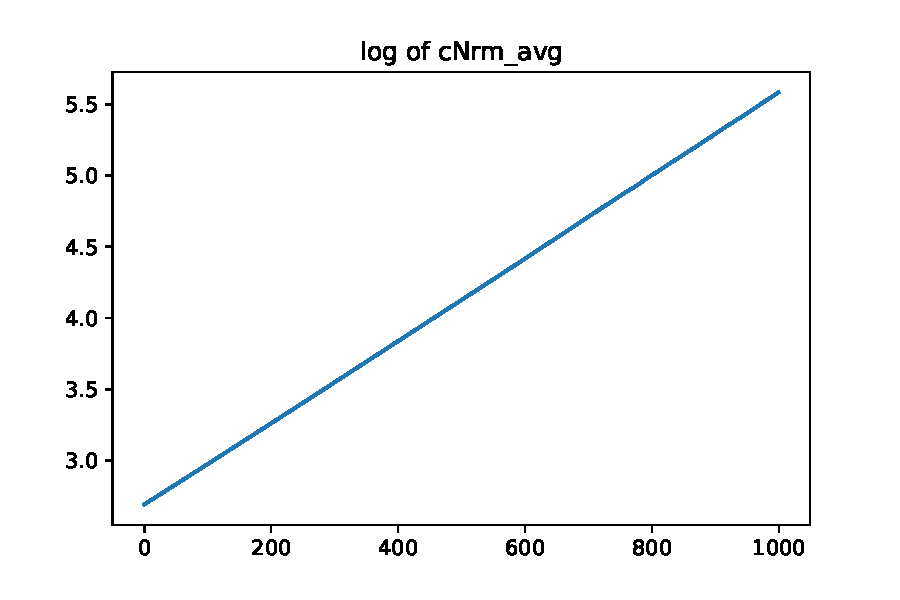
\includegraphics[width=4in]{Figures/logcNrm}
  }
  \caption{Appendix: $\log ~\mathfrak{c}$ Appears to Grow Linearly}
  \label{fig:logcNrm}
\end{figure}
\begin{figure}[ht]
  \centerline{
    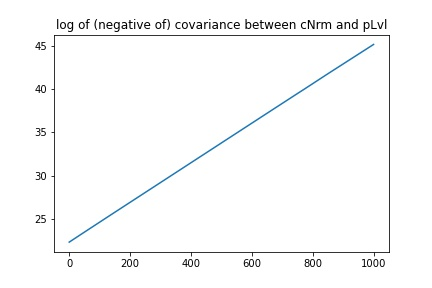
\includegraphics[width=4in]{Figures/logcov}
  }
  \caption{Appendix: $\log ~(-\cov(\cNrm,\permLvl))$ Appears to Grow Linearly}
  \label{fig:logcov}
\end{figure}


\end{document}
\endinput

% Local Variables:
% eval: (setq TeX-command-list  (assq-delete-all (car (assoc "BibTeX" TeX-command-list)) TeX-command-list))
% eval: (setq TeX-command-list  (assq-delete-all (car (assoc "BibTeX" TeX-command-list)) TeX-command-list))
% eval: (setq TeX-command-list  (assq-delete-all (car (assoc "BibTeX" TeX-command-list)) TeX-command-list))
% eval: (setq TeX-command-list  (assq-delete-all (car (assoc "BibTeX" TeX-command-list)) TeX-command-list))
% eval: (setq TeX-command-list  (assq-delete-all (car (assoc "Biber"  TeX-command-list)) TeX-command-list))
% eval: (add-to-list 'TeX-command-list '("BibTeX" "bibtex.%s" TeX-run-BibTeX nil t                                                                              :help "Run BibTeX") t)
% eval: (add-to-list 'TeX-command-list '("BibTeX" "bibtex.%s" TeX-run-BibTeX nil (plain-tex-mode latex-mode doctex-mode ams-tex-mode texinfo-mode context-mode) :help "Run BibTeX") t)
% TeX-PDF-mode: t
% TeX-file-line-error: t
% TeX-debug-warnings: t
% LaTeX-command-style: (("" "%(PDF)%(latex) %(file-line-error) %(extraopts) -output-directory=. %S%(PDFout)"))
% TeX-source-correlate-mode: t
% TeX-parse-self: t
% eval: (cond ((string-equal system-type "darwin") (progn (setq TeX-view-program-list '(("Skim" "/Applications/Skim.app/Contents/SharedSupport/displayline -b %n %o %b"))))))
% eval: (cond ((string-equal system-type "gnu/linux") (progn (setq TeX-view-program-list '(("Evince" "evince --page-index=%(outpage).%o"))))))
% eval: (cond ((string-equal system-type "gnu/linux") (progn (setq TeX-view-program-selection '((output-pdf "Evince"))))))
% TeX-parse-all-errors: t
% End:
